%--------------------------------------------------------------------------
\begin{frame}{Mathematical Modelling and Numerical Simulation}
%--------------------------------------------------------------------------
  \begin{itemize}
  \item \alert{Mathematical Model}: representation of physical reality
    that is suitable for \textit{analysis} and \textit{calculation}
  \item \alert{Numerical Simulation} allows us to \textit{calculate the
    solution of a model} in a computer and therefore to simulate
    physical reality
  \end{itemize}
  \medskip
  In this work\dots
  \smallskip
  \begin{itemize}
  \item models defined by \textbf{PDEs} (Partial Differential Equations)
  \item we shall introduce models of \textit{increasing complexity}
  \item targets:
    \begin{itemize}
    \item to explore and \textit{analyze} models in large-scale
      \textbf{Oceanography}
    \item to develop \textit{numerical methods} for simulate
      ocean flow
    \end{itemize}
  \end{itemize}
\end{frame}

%--------------------------------------------------------------------------
\begin{frame}{A First Example of Modelling}
%--------------------------------------------------------------------------
  Modelling requires \alert{great effort} for an applied mathematician
  \begin{itemize}
  \item Thorough knowledge of \llaveizq{\textit{mathematics}\\\textit{scientific discipline}}
  \item To communicate with other scientists, to select the adequate
    model between different possibilities, to simplify models which
    are too complex\dots
  \item In later stage, also \textit{computing skills}
  \end{itemize}

  \bigskip
  We start describing a simple model: the \alert{Heat Equation}
\end{frame}

\SetEmptyBackground
%--------------------------------------------------------------------------
\begin{frame}
%--------------------------------------------------------------------------
  Let
  \begin{itemize}
  \item $\Omega\subset\Rset^N$, \quad ($N=1,2,3$), \ open spatial domain \tiragris{occupied by a
      homogeneous, isotropic, heat conductor material}
  \item $\xx=(x_1,\dots,x_N) \in \Omega$: \textit{space} variable, \quad $t\in (0,T)$: \textit{time} variable
  \item \textit{Temperature}: unknown function,
    \begin{align*}
    u:\Omega\times (0,T) \to \Rset, \\
      (\xx,t) \mapsto u(\xx,t).
    \end{align*}
    \vspace{-1em}
    \pause
  \item \textit{Heat source}: a given function, $f(\xx,t)$
    \vspace{0.66em}
  \item Using physical laws (see e.g.~\cite{allaire:2007}),
    \begin{itemize}
    \item conservation of energy (of heat),
    \item quantity of heat is proportional to temperature: $c u$, \ $c\in\Rset$,
    \item heat flux proportional to temperature gradient: $q=-k\grad u$, $k\in\Rset$,
      \tiragris{\tiny $c$, $k$: physical
        constants (dependent on material), called ``specific heat'' and ``thermal conductivity''}
    \end{itemize}
  \item \dots and some mathematical theory (Gauss theorem), we arrive to\dots
  \end{itemize}
\end{frame}

\SetDefaultBackground
%--------------------------------------------------------------------------
\begin{frame}{The Heat Equation}
%--------------------------------------------------------------------------
  \begin{itemize}
  \item ... we arrive to the following \textbf{PDE} in $\Omega$:
    \begin{BlockNoTitle}
      \begin{equation*}
        c\, \framedmath<2>{\dt u} - k\, \framedmath<3>{\Delta u} = f
        \qquad \soften{\text{in} \quad \Omega\times (0,T),}
      \end{equation*}
    \end{BlockNoTitle}
    where:
    \begin{itemize}
    \item $\framedmath<2>{\dt u} = \frac{\partial u}{\partial t}$
      \quad (time partial derivative)
    \item
      $\framedmath<3>{\Delta u} = \sum_{i=1}^N \frac{\partial^2
        u}{\partial x_i^2}$ \quad (Laplacian operator)
    \end{itemize}
    \bigskip
    \item<4-> We must add an \textbf{initial condition}
      \soften{(state of the model at time $t=0$)}:
      \begin{BlockNoTitle}
        \begin{equation*}
          u(\xx,0) = u_0(\xx), \soften{ \qquad \forall \xx\in\Omega}
        \end{equation*}
      \end{BlockNoTitle}

    \item<4->
      And also \textbf{boundary conditions}
      \soften{(evolution of the model on the boundary,
        $\xx\in\partial\Omega$)}\dots
  \end{itemize}
\end{frame}

%--------------------------------------------------------------------------
\begin{frame}{Boundary Conditions {\small (to select depending on physical context)}}
%--------------------------------------------------------------------------
  % \vspace{-1.5em}
  % Different possibilities to select \soften{ (depending on physical context)}:
  % \medskip
  \begin{enumerate}
  \item \alert{Dirichlet} boundary condition:
    \begin{BlockNoTitle}
      \begin{equation*}
        u(\xx,t)=0, \quad \forall \xx\in\partial\Omega, \quad \forall t\in(0,T)
      \end{equation*}
    \end{BlockNoTitle}
  \item \alert{Neumman} boundary condition:
    \begin{BlockNoTitle}
      \begin{equation*}
        \partial_{\nn} u(\xx,t) := \grad u(\xx,t)\cdot\nn = 0,
      \end{equation*}
    \end{BlockNoTitle}
    {\small\hfill
     where $\grad u =$ gradient vector and $\nn=$ unit outward vector normal to $\Omega$.}
    \smallskip
    \tiragris{\scriptsize{}
        \textbf{Interpretation}: No heat flux across $\partial\Omega$ (domain isolated from the exterior)}
  \item \alert{Robin} (or Fourier) boundary condition
    \begin{BlockNoTitle}
      \begin{equation*}
        \partial_{\nn} u(\xx,t) + \alpha u(\xx,t) = 0,
      \end{equation*}
    \end{BlockNoTitle}
    {\small\hfill where $\alpha>0$ is a given constant}
    \tiragris{\scriptsize
      \begin{tabular}{r}
      \textbf{Interpretation}: Heat flux trough $\partial\Omega$ is proportional to
        the difference \\ of temperature between exterior and interior
      \end{tabular}
    }
  \end{enumerate}
\end{frame}

%--------------------------------------------------------------------------
\begin{frame}{The Heat Equation}
%--------------------------------------------------------------------------
  We can summarize in the following problem: find $u(\xx,t)$ such that
  \begin{BlockNoTitle}%
    \begin{tabular}[t]{l|>{$}l<{$}l}
       \rotatebox[origin=c]{40}{\small \heatProblem}
      &
        \begin{aligned}%
          \dt u - \nu\, \Delta u &= f
          \qquad \text{in} \ \Omega\times (0,T),
          \\\noalign{\smallskip}
          u|_{t=0} &= u_0
          \qquad \text{in}\ \Omega,
          \\\noalign{\smallskip}
          u&=0
          \qquad \text{on}\ \partial\Omega \times (0,T),
        \end{aligned}
    \end{tabular}
  \end{BlockNoTitle}
  where $\nu=k/c>0$ (viscosity coefficient) and we fixed Dirichlet B.C.
  \pause
  \small
  \begin{remark}
    This problem has a universal character and is applied to model \structure{many phenomena}:
    \begin{itemize}
    \item Heat propagation
    \item Diffusion of a density or concentration (of biological
      species, of pollution,\dots)
    \item In finance, value of an option to buy a stock
    \item \dots
    \end{itemize}
  \end{remark}
\end{frame}

%--------------------------------------------------------------------------
\begin{frame}{The Poisson Problem}
%--------------------------------------------------------------------------
  For certain choices of the source term, $f(x)$, Heat Equation reaches a
  \alert{\textbf{steady}} or (\textbf{stationary}) state, that is
  $$
  u(\xx,t) \longrightarrow u_\infty(\xx) \quad\mbox{as}\quad t\to\infty.
  $$
  Often it is interesting to calculate the steady state directly, solving:
  \begin{BlockNoTitle}%
    \begin{tabular}[t]{l|>{$}l<{$}l}
       \rotatebox[origin=c]{30}{\small \poissonProblem}
      &
        \begin{aligned}%
          \Delta u &= f
          \qquad \text{in} \ \Omega,
          \\\noalign{\smallskip}
          u&=0
          \qquad \text{on}\ \partial\Omega.
        \end{aligned}
    \end{tabular}
  \end{BlockNoTitle}
  \medskip
  \pause
  Now we are about to use this simpler problem as example for:
  \smallskip
  \begin{enumerate}
  \item \emph{Analysis} of the model (including existence and uniqueness of solution) and
  \item \emph{Numerical simulation} (calculating the solution).
\end{enumerate}
\end{frame}

%--------------------------------------------------------------------------
\begin{frame}{Variational Formulation of \poissonProblem}
%--------------------------------------------------------------------------
  \small
  \begin{proposition}
  Let
  $$
  X=\{ \Phi\in C^1(\overline\Omega) \st \Phi=0 \quad \mbox{on } \partial\Omega\}.
  $$
  A function $u\in C^2(\Omega)$ is a solution of \poissonProblem $\mathbf\Longleftrightarrow$ $u\in X$ and satisfies:
  \begin{equation}
    \tag{\ensuremath{P_V}}
    \int_\Omega \grad u(\xx) \grad v(\xx) d\xx = \int_\Omega f(\xx) v(\xx) d\xx \quad \forall v\in X.
    \label{eq:poisson.variational}
  \end{equation}
  \end{proposition}
  \begin{itemize}
  \item Proof: follows from Green's formula (integration by parts).
  \item Problem (\ref{eq:poisson.variational}) is called
    \alert{\textbf{Variational Formulation}} of \poissonProblem.
  \item $v$ is called \textbf{test function}.
  \item (\ref{eq:poisson.variational}) only requires
    $u\in C^1(\Omega)$. In this sense it is \textbf{weaker} than ``classical
    formulation'' of \poissonProblem, which requires $u\in C^2(\Omega)$.
  \item $\Rightarrow$ we suspect that it is \textbf{easier to solve}
    (\ref{eq:poisson.variational}) than ``classical formulation''.
  \end{itemize}
  \vspace{-1em}
  \begin{BlockNoTitle}
    \begin{center}
      \textbf{Idea:} Is possible to develop a theory for
      well-posedness of~(\ref{eq:poisson.variational})? \ \dots
    \end{center}
  \end{BlockNoTitle}
\end{frame}

%--------------------------------------------------------------------------
\begin{frame}{Abstract framework}
%--------------------------------------------------------------------------
  \begin{itemize}
  \item Reformulation of (\ref{eq:poisson.variational}): find
    $u\in X$ such that
    \begin{BlockNoTitle}
      \begin{equation}
        \tag{\ensuremath{P_V}}
        a(u,v) = L(v) \quad \forall v\in
        X,\label{eq:abstract.variational}
      \end{equation}
    \end{BlockNoTitle}
    were $a(\cdot,\cdot)$ and $L(\cdot)$ \soften{are the following} bilinear and linear forms:
    \begin{equation*}
      a(u,v) = \int_\Omega \grad u \grad v, \qquad
      L(v) = \int_\Omega f  v.
    \end{equation*}

  \item There \alert{\textbf{exists a powerful theory}}
    (\structure{Lax-Milgram}) for analysing abstract variational
    formulations like~(\ref{eq:abstract.variational}).

  \item \soften{However, this theory} \textbf{only works for Hilbert spaces}. \soften{And}
    $$
    X=\{ \Phi\in C^1(\overline\Omega) \st \Phi=0 \quad \mbox{on } \partial\Omega\}
    $$
    is \textbf{not a Hilbert space} \soften{(equipped with  the "natural" scalar product for this problem)}.
  \item \soften{We therefore must} \alert{\textbf{replace $X$ with a Hilbert space}, $V$}.
  \end{itemize}
\end{frame}

%--------------------------------------------------------------------------
\begin{frame}{Lax-Milgram Theory}
%--------------------------------------------------------------------------
  \small
  Let $V$ a Hilbert space.
  \soften{Consider the abstract problem:}
  Find $u\in V$ such that
    \begin{BlockNoTitle}
      \begin{equation}
        \tag{\ensuremath{P_V}}
        a(u,v) = L(v) \quad \forall v\in V,
        \label{eq:abstract.variational.hilbert}
      \end{equation}
    \end{BlockNoTitle}
    \soften{and the following} hypothesis:
    \begin{enumerate}
    \item $L(\cdot)$ is \textbf{linear} and \textbf{continuous}, \soften{i.e.} $\exists C>0$ \soften{such that:}
      \label{item:1}
      \begin{equation*}
        |L(v)|\le C \norm[]{v} \quad \forall v\in V.
      \end{equation*}
    \item $a(\cdot,\cdot)$ is \textbf{bilinear} and \textbf{continuous}, \soften{i.e.} $\exists M>0$ \soften{such that:}
      \label{item:2}
      \begin{equation*}
        |a(v,w)|\le M \norm[]{v}\norm[]{w} \quad\forall v,w\in V,
      \end{equation*}
    \item $a(\cdot,\cdot)$ is \textbf{coercive}, \soften{i.e.} $\exists \nu>0$ \soften{such that:}
      \label{item:3}
      \begin{equation*}
        |a(v,v)| \ge \nu  \norm[]{v}^2 \quad\forall v\in V,
      \end{equation*}
    \end{enumerate}
    \begin{theorem}[Lax-Milgram]
      Under previous
      hypothesis,~\alert{(\ref{eq:abstract.variational.hilbert})} is
        well posed, i.e., it \alert{\textbf{has a unique solution}} which
      depends continuously on $L$.
    \end{theorem}
\end{frame}

%--------------------------------------------------------------------------
\begin{frame}{Sobolev spaces}
%--------------------------------------------------------------------------
  \small
  \soften{Some results from \textbf{functional analysis}:}
  \begin{itemize}
  \setlength\itemsep{0.5em}
  \item<1->
    $L^p(\Omega)=\{ f: \Omega \to \Rset \quad \text{measurable} \st
    \alert{\int_\Omega |f(\xx)|^p < +\infty} \} \quad p \in [1,+\infty)$
    \begin{itemize}
      \setlength\itemsep{0.3em}
      \scriptsize
    \item $L^p(\Omega)$ is a Banach space for
      $\norm[L^p(\Omega)]{f}=\left(\int_\Omega|f(\xx)|^p\right)^{1/p}$
    \item $L^2(\Omega)$ is a Hilbert space for $(f,g)_{L^2(\Omega)}=\int_\Omega f(\xx) g(\xx) d\xx$
    \end{itemize}

  \item<2->
    $ H^m(\Omega) = \{ f\in L^2(\Omega) \st \text{\alert{weak derivatives} of
      order $|\alpha| \le m$ are \alert{in} } \alert{L^2(\Omega)} \} $
    \begin{itemize}
      \setlength\itemsep{0.3em}
      \scriptsize
    \item Hilbert space for
      $(f,g)_{H^m(\Omega)}=\sum_{|\alpha|\le m} \int_\Omega D^\alpha f
      \; D^\alpha g \,d\xx$.
      \par \soften{ which induces the norm:} \quad
      $\norm[H^m(\Omega)]{f}=\left(\sum_{|\alpha|\le m} \int_\Omega|D^\alpha f(\xx)|^2\right)^{1/2}$
      \item $C^\infty(\overline\Omega) \subset H^m(\Omega)$, dense inclusion.
    \end{itemize}

  \item<3-> \alert{$H_0^1(\Omega) = \{ v \in H^1(\Omega) \st v|_{\partial\Omega}=0 \}$}
     \hfill\soften{ (sense of $v|_{\partial\Omega}=0$ ? Trace theory)}
    \begin{itemize}
      \setlength\itemsep{0.3em}
      \scriptsize
    \item Hilbert space for
      $(f,g)_{H_0^1(\Omega)}=\int_\Omega \grad f \; \grad g \, d\xx $
      \par \soften{ which induces the norm:} \quad
      $\norm[H_0^1(\Omega)]{f}=\left(\int_\Omega|\grad f|^2\, d\xx\right)^{1/2}$
    \item $D(\Omega) =\{ \small \Phi\in C^\infty(\Omega) \st \text{ soporte compacto} \}
      \subset H_0^1(\Omega)$, dense.
       \small
     $$\Rightarrow
      D(\Omega) \subset \alert{X=\{ \Phi\in C^1(\overline\Omega) \st \Phi=0 \quad \mbox{on
      } \partial\Omega\} \subset H_0^1(\Omega)} \text{, dense}.$$
    \end{itemize}
  \end{itemize}
\end{frame}

%--------------------------------------------------------------------------
\begin{frame}{Well-posedness of the Poisson Problem}
%--------------------------------------------------------------------------
  \begin{theorem}
    Let $\Omega \subset \Rset^N$ open, bounded set. Take $f\in L^2(\Omega)$.
    \begin{enumerate}
    \item \alert{$\exists! u \in V=H_0^1(\Omega)$ solution} of the variational formulation
      \begin{equation}
        \tag{\ensuremath{P_V}}
        \int_\Omega \grad u \, \grad v \,d\xx = \int_\Omega f\, v \, d\xx \quad \forall v\in V.
        \label{eq:1}
      \end{equation}
    \item Further, it \alert{depends continuously on the data}, i.e., $\exists C>0$ such that
      $$
      \norm[H_0^1(\Omega)]{u} \le C \norm[L^2(\Omega)]{f}.
      $$
    \item If $\Omega$ is an open set of class $C^{m+2}$ and
      $f\in H^m(\Omega)$ with $m>N/2$, then the solution $u$
      of~(\ref{eq:1}) is a \alert{\textbf{strong} or \textbf{classical solution}} i.e. it verfies
      $$
      u\in C^2(\overline\Omega), \qquad -\Delta u(\xx) = f(\xx) \quad \forall \xx\in\Omega, \quad u|_{\partial\Omega}=0.
      $$
    \end{enumerate}
  \end{theorem}
  \scriptsize \textbf{Proof}: (1) and (2) are consequence of
  \structure{\textbf{Lax-Milgram}} Theorem. (3) requires more \structure{functional
    analysis}, see e.g.~\cite{brezis:2017,allaire:2007}.
\end{frame}

%--------------------------------------------------------------------------
\begin{frame}{Numerical Simulation}
%--------------------------------------------------------------------------

Construction of any numerical method for solving a (steady) PDE requires to consider:

\bigskip

\begin{enumerate}
  \setlength\itemsep{1.2em}
\item How to represent the solution $u(\xx,t)$ by an
  \textit{approximate solution} $u_h(\xx,t)$?
\item In which sense the approximate solution $u_h (\xx,t)$
  satisfies the PDE?
\end{enumerate}
\end{frame}

%--------------------------------------------------------------------------
\begin{frame}{Finite Difference Method}
%--------------------------------------------------------------------------
Simpler numerical method for PDE

Example: the \alert{Poisson problem} in
$\Omega=(0,1)\times (0,1) \subset\Rset^2$:

\begin{enumerate}
  \setlength\itemsep{1.1em}
\item We consider the mesh \structure{$\overline \Omega_h = \{ (x_i,y_j)=(ih,jh) \st 0 \le i,j \le M \} $}
and \alert{define $u_h(\xx)$ by} \soften{piecewise interpolation of the approximations}
$$
\alert{u^h_{ij}\simeq u(x_i,y_j)}.
$$
\item Partial derivatives are approximated \structure{on each interior node $(x_i,y_j)$} as incremental quotients:
  \begin{BlockNoTitle}
    \vspace{-1.5em}
    \begin{multline*}
      -\Delta u(x_i,y_j) = -\partial^2_{xx}u(x_i,y_j)
      -\partial^2_{yy}u(x_i,y_j)\simeq
      \\
      -\frac{u_{i-1,j}-2u_{ij}+u_{i+1,j}}{h^2}
      -\frac{u_{i,j-1}-2u_{ij}+u_{i,j+1}}{h^2} = f(x_i,x_j).
    \end{multline*}
  \end{BlockNoTitle}
  + B.C. $\Rightarrow$ \textbf{linear equations system}, $(M-1)^2$ equations and unknowns.
\end{enumerate}

\end{frame}

%--------------------------------------------------------------------------
\begin{frame}{Finite Element Method (FEM)}
%--------------------------------------------------------------------------
  \begin{enumerate}
  \item We approximate $\overline\Omega$ by a \alert{triangulation
    ${\cal T}_h= \{K_i\}_{i}^M$}. Then select a polynomial order,
    \alert{$k\in\Nset$}, and define the space
    \begin{BlockNoTitle}
      \vspace{-0.5em}
      $$
      \alert{V_h} = \big\{ v_h\in C^0(\overline\Omega) \;\st\;
      v_h|_{K_i}\in\mathbb{P}_k, \ \forall K_i \in {\cal T}, \quad
      v_h|_{\partial\Omega}=0 \big\}.
      $$
    \end{BlockNoTitle}

    \medskip
    This kind of approximations shall also be denoted as \alert{\P{k}}.
    \medskip

    \setlength{\tabcolsep}{1.5em}
    \begin{center}
      \begin{tabular}{cc}
        \centering
        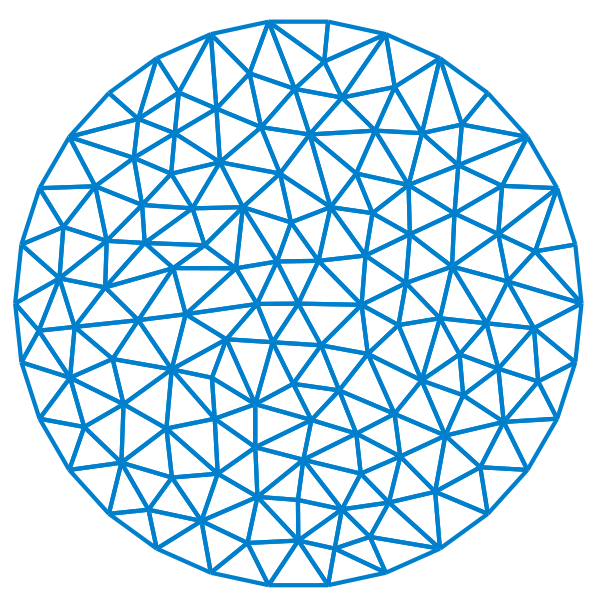
\includegraphics[height=0.25\linewidth]{img/FE_triangulation}
        &
          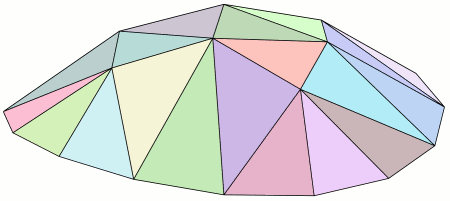
\includegraphics[height=0.18\linewidth]{img/FE_function_3d}
        \\
        {\scriptsize  Triangulation of $\overline\Omega$}
        &
          {\scriptsize Function $u_h \in V_h$ (\P1 approximation)}
      \end{tabular}
    \end{center}

  \end{enumerate}
\end{frame}

%--------------------------------------------------------------------------
\begin{frame}{Finite Element Method (FEM) \quad \soften{(for the Poisson Problem)}}
%--------------------------------------------------------------------------
  \begin{enumerate}
    \setcounter{enumi}{1}
  \item We \alert{approximate the \textbf{variational
        formulation}} of the Poisson problem as follows: \alert{find
    $u_h\in V_h$} such that:
    \begin{BlockNoTitle}
      \begin{equation}
        \tag{\ensuremath{P_{\text{FEM}}}}
        \int_\Omega \grad u_h(\xx) \grad v_h(\xx) d\xx = \int_\Omega f(\xx) v_h(\xx) d\xx \quad \forall v_h\in V_h.
        \label{eq:pb.poisson.FE}
      \end{equation}
    \end{BlockNoTitle}
  \end{enumerate}

 \bigskip

  \begin{proposition}
    \begin{itemize}
    \setlength\itemsep{0.7em}
    \item \alert{$V_h$} is a \alert{finite-dimensional} subspace of
        $V=\alert{H_0^1(\Omega)}$
    \item (\ref{eq:pb.poisson.FE}) has a \alert{\textbf{unique
          solution}}, $\uh$. In fact, it is \alert{equivalent to a
        linear system} with sparse, symmetric and positive defined
      matrix.
    \end{itemize}
  \end{proposition}

  \medskip\small
  $\dim(V_h)$ is known as the \textit{number of degrees of freedom} of $V_h$.
\end{frame}


%--------------------------------------------------------------------------
\begin{frame}{Convergence and Error Orders}
%--------------------------------------------------------------------------
  \begin{itemize}
    \setlength\itemsep{0.7em}
  \item Let ${\cal T}_h$ ($h\to 0$) \soften{be a sequence of regular} meshes of $\Omega$ and let
    \medskip
    \begin{itemize}
    \setlength\itemsep{0.3em}
    \item $u\in H_0^1(\Omega)$: solution of the Poisson problem and
    \item $u_h\in V_h$: its $\P{k}$ FE approximation \soften{(solution of~(\ref{eq:pb.poisson.FE}))}.
    \end{itemize}
    Then
    $$
    \alert{\lim_{h\to 0} \norm[H^1(\Omega)]{u-u_h} = 0}.
    $$
  \item Moreover, if $u\in H^{k+1}$ and $k+1>N/2$, one has \soften{the
      following error estimates}%
    \footnote{\soften{Where $C$ is a constant (independent of $h$ and
        $u$). Regularity of $\partial\Omega$ or convexity for $n=2$ is
        required for~(\ref{eq:error.estimate.L2}) see
        e.g.~\cite{Brenner-Scott:08}.}}:
    \begin{align}
      \label{eq:error.estimate.H1}
      \norm[\alert{H^1}(\Omega)]{u-u_h} &\le C \, \alert{h^k} \, \norm[H^{k+1}(\Omega)]{u}
      \\
      \label{eq:error.estimate.L2}
      \norm[\alert{L^2}(\Omega)]{u-u_h} &\le C \, \alert{h^{k+1}} \, \norm[H^{k+1}(\Omega)]{u}
    \end{align}
    We say \alert{\textbf{optimal error estimates}}.
  \end{itemize}
\end{frame}

\begin{frame}{Time Dependent Problems}
  \begin{small}
    Example: the \textbf{Heat equation}:
  \end{small}
  \begin{BlockNoTitle}%
    \begin{equation*}
        \begin{aligned}%
          \dt u - \nu\, \Delta u &= f
          \qquad \text{in} \ \Omega\times (0,T),
          \\[0.1em]
          u|_{t=0} &= u_0
          \qquad \text{in }\ \Omega,
          \\[0.1em]
          u&=0
          \qquad \text{on }\ \partial\Omega \times (0,T).
        \end{aligned}
      \end{equation*}
  \end{BlockNoTitle}
  \begin{theorem}
    Let $\Omega$ be an regular open set of $\Rset^N$. Take a final
    time $T>0$, initial data $u_0\in L^2(\Omega)$ and a source term
    $f\in L_2( (0,T); L^2(\Omega))$.
    \par\medskip
    Then \alert{the heat equation has a unique solution}
    $$
    u\in L^2( (0,T); H_0^1(\Omega)) \ \cap \ C([0,T];L^2(\Omega))
    $$
    \soften{...and energy estimates are verified.}
    % \par\medskip
    % Further, there exists $C>0$ (which only depends on $\Omega$) such that
    % $$
    % \norm[L^2(\Omega)]{u(\cdot,t)}^2
    % $$
  \end{theorem}
  \soften{\small\textbf{Proof}: functional analysis for evolution problems, see e.g.~\cite{allaire:2007}.}
\end{frame}


\begin{frame}{Numerical Methods for Time Dependent Problems}
  \small
  \textbf{Idea}: \soften{Numerical scheme for Cauchy problems (ODE), e.g. Implicit Euler}
  \smallskip
  \begin{itemize}
    \setlength{\itemsep}{0.3em}
  \item \small Partition of $[0,T]$: \
    $0=t_0<t_1<\cdots<t_n=T$, \quad $k=T/n$ \soften{\small (time
      step)}
  \item At each time step, $t_{k}$, we look for
     \alert{$u^{m+1}$} \soften{such that}
    % \vfill
     \begin{BlockNoTitle}%
      \begin{tabular}[t]{>{\hspace{3em}}l|l}
        \rotatebox[origin=c]{30}{\framedmath<2>{Implicit} Euler}
        &$\displaystyle
          \begin{aligned}
            \frac{\framedmath<2>{u^{m+1}}-u^m}{k} - \nu\Delta
            \framedmath<2>{u^{m+1}} &= f^{m+1} \qquad \text{in}\ \Omega,
            \\
            u&=0
            \qquad \text{on}\ \partial\Omega \times (0,T).
          \end{aligned}
               $
      \end{tabular}
    \end{BlockNoTitle}
  \end{itemize}
  \pause
  \alert{Variational formulation\dots}
  \begin{enumerate}
    \setlength{\itemsep}{0.5em}
  \item $u^0=u_0 \in H_0^1(\Omega)$
  \item Given $u^m\in H_0^1(\Omega)$, find \alert{$u^{m+1}\in H_0^1(\Omega)$} \soften{such that}
    $$ a(u^{m+1},v)= L(v) \quad \forall v\in H_0^1(\Omega), $$
  \end{enumerate}
  where, \soften{for all $u,v \in H_0^1(\Omega)$}:
  $$
  a(u,v) = \int_\Omega \big(u\,v+ k \nu \,\grad u \,\grad v\big), \quad L(v)=\int_\Omega \big( u^m  + k\, f^{m+1} \big) v.
  $$
\end{frame}

\begin{frame}{The Stokes System}
  It models the flow of a \textit{\structure{viscous}}
  \textit{\structure{incompressible}} \textbf{fluid}, with
  ``\textit{\structure{small velocity}}''%
  \footnote{\scriptsize {I.e. the Reynolds number is small:
    $$
    \text{Re}:=\frac{\text{intertial forces}}{\text{viscous forces}}
    =\frac{vL}{\nu} \ll 1.
    $$
  }}
\begin{BlockNoTitle}
  \vspace{-1.2em}
  \begin{align*}
    \partial_t \uu - \nu \Delta\uu + \grad\pp &= \ff \quad\text{in }\Omega\times(0,T)
    \\
    \div\uu &= 0 \quad\text{in }\Omega\times (0,T)
    \\
    u &= 0 \quad\text{on } \partial\Omega\times (0,T), \quad u|_{t=0} = u_0 \quad\text{in } \Omega
  \end{align*}
\end{BlockNoTitle}
\vspace{-0.5em}
% where:
\begin{small}
  \begin{itemize}
  \setlength{\itemsep}{-0.1em}
\item Unknowns: \emph{\alert{velocity}}, \
  $\uu(\xx,t)=(u_1(\xx,t),\dots,u_N(\xx,t))$ \ and
  \emph{\alert{pressure}}, \ $p(\xx,t)$
  \item First equation (\alert{conservation of momentum}) is vectorial ($N$ equations)
  \item Last equation (\alert{incompressibility condition}) couples velocity unknowns!
    $$\div\uu = \partial_{x_1}u_1+\cdots+\partial_{x_N}u_N=0.$$
  \item \scriptsize{More general equations (for arbitrary Reynolds
      number) are the \alert{Navier--Stokes} equations.}
  \end{itemize}
\end{small}
\end{frame}

\begin{frame}{Analysis of Steady Stokes Equations}
  \begin{small}
    Let us focus on the stationary case:
  \end{small}
  \begin{BlockNoTitle}
    \vspace{-0.3em}
    \begin{tabular}[t]{l|l}
       \rotatebox[origin=c]{40}{\small \steadyStokes}
      &
        $
    \begin{aligned}
       - \nu \Delta\uu + \grad\pp &= \ff \quad\text{in }\Omega\times(0,T),
      \\
      \div\uu &= 0 \quad\text{in }\Omega\times (0,T),
      \\
      u &= 0 \quad\text{on } \partial\Omega\times (0,T).
    \end{aligned}
          $
    \end{tabular}
  \end{BlockNoTitle}
  Mixed \alert{\textbf{variational formulation}}: find
  $(\uu,\pp)\in \mathbf{U}\times P$ such that
  \begin{BlockNoTitle}
    \vspace{-1.3em}
    \begin{align*}
    a(\uu,\bu) + b(\bu,\pp) &= L(\bu), & \forall \bu\in \mathbf{U},
    \\
    b(\uu,\bp) &= 0 & \forall\bp\in P,
    \end{align*}
  \end{BlockNoTitle}
  \medskip
  where \quad \alert{$\mathbf{U}=\big(H_0^1(\Omega)\big)^N$}, \quad
  \alert{$P=\{p\in L^2(\Omega)/ \int_\Omega p=0 \}$} \quad and
  \vspace{-0.3em}
  \begin{align*}
    a(\uu,\bu)&=\int_\Omega \grad\uu\;\grad \bu \ := \sum_{i=1}^N \int_\Omega \grad u_i \cdot \grad \overline u_i,
    \\
    b(\bu,\pp)&=-\int_\Omega p \; \div\bu, \qquad L(\bu)=\int_\omega \ff\cdot\bu
  \end{align*}
\end{frame}

\SetEmptyBackground
\begin{frame}
    \begin{theorem}
      Let $\Omega\subset\Rset^N$ be a regular open bounded connected set of
      class $C^1$ and let $f\in L^2(\Omega)^N$.
      \par\smallskip Then \alert{exists a unique
      (weak) solution of \steadyStokes}, $(\uu,p)\in \mathbf{U}\times P$.
    \end{theorem}
    \begin{proof}
      \small
      \begin{itemize}
        \setlength{\itemsep}{0.5em}
      \item \small{Not possible to apply Lax-Milgram to the ``\textit{global bilinear
        form}'' (not coercive on $\textbf{U}\times P$)}
        \vspace{-0.5em}
        $$
        {\cal A}((\uu,\pp),(\bu,\bp))=a(\uu,\bu)+b(\bu,\pp)+b(\uu,\bp).
        $$
        \vspace{-1.5em}
      \item But the following conditions hold:
        \begin{enumerate}
        \item  \alert{\textbf{Inf-Sup
              Condition}}: $\exists\beta>0$ such that
          \begin{equation}
            \tag{IS}
            \sup_{\bu\in\mathbf{U}}\frac{b(\bu,p)}{\norm[\mathbf{U}]{\bu}} \ge \beta \norm[L^2(\Omega)]{p}, \quad \forall p\in P.
          \end{equation}
          \vspace{-0.5em}
        \item $a(\cdot,\cdot)$ is coercive on \textbf{U}.
        \end{enumerate}
      \item And they are sufficient for a ``generalized saddle point result''  \cite{Boffi-Brezzi-Fortin:08}
      \end{itemize}
    \end{proof}
\end{frame}

\SetDefaultBackground
\begin{frame}{Finite Elements for the Stokes problem}
  Let $\Uh\subset \mathbf{U}$ and $\Ph\subset P$ finite element spaces on a mesh \Th
  % \begin{align*}
  %   \Uh &= \big\{\uh \in C^0(\Omega) \ \st\ \uh|_{K_i}\in \mathbb{P}_{\alert{k}}^N \quad \forall K_i\in \Th \quad \uh|_{\partial\Omega}=0\big\},
  %   \\
  %   \Ph &= \big\{\ph \in C^0(\Omega) \ \st\ \ph|_{K_i}\in \mathbb{P}_{\alert{\ell}}^N \quad \forall K_i\in \Th\}.
  % \end{align*}
  and consider the \alert{discrete variational formulation}:
  \begin{BlockNoTitle}
    \vspace{-1em}
    \begin{align*}
      a(\uh,\buh) + b(\buh,\ph) &= L(\vh) & \forall \buh\in \Uh,
      \\
      b(\uh,\bph) &=0 & \forall \bph \in \Ph.
    \end{align*}
  \end{BlockNoTitle}

  The \soften{(continuous)} inf-sup condition is not inherited by \Uh, \Ph. One has:

  \begin{theorem}
    For \alert{existence and uniqueness} of solution of discrete
    formulation, it is necessary and sufficient that \Uh, \Ph verify
    the following \alert{\textbf{Discrete Inf-Sup Condition}}: $\exists \gamma>0$ such that
    \begin{equation}
      \tag{\ensuremath{IS_h}}
      \sup_{\buh\in\Uh}\frac{b(\buh,\bph)}{\norm[\Uh]{\buh}} \ge \gamma \norm[L^2(\Omega)]{\bph}, \quad \forall \bph\in \Ph.
      \label{eq:stokes:ISh}
    \end{equation}
  \end{theorem}
  \soften{\textbf{Proof}: See e.g.~\cite{Brenner-Scott:08}.}
\end{frame}

\begin{frame}{Usual FE Spaces Verifying~(\ref{eq:stokes:ISh})}
  \begin{itemize}
  \item \textbf{Taylor-Hood} elements: \alert{$\P2/\P1$}, i.e.:
    \begin{align*}
      \Uh &= \big\{\uh \in C^0(\Omega) \ \st\ \uh|_{K_i}\in \alert{\mathbb{P}_{2}}^N \quad \forall K_i\in \Th \quad \uh|_{\partial\Omega}=0\big\}
      \\
      \Ph &= \big\{\ph \in C^0(\Omega) \ \st\ \ph|_{K_i}\in \alert{\mathbb{P}_{1}} \quad \forall K_i\in \Th \quad \int_\Omega \ph=0\}
    \end{align*}

  \item
    \textbf{Mini-element}: \alert{$\P{1,b} / \P1$}:
    \par Let $\widehat b$ denote a \alert{bubble function} i.e. \llaveizq{$1$
      \quad in \ the barycenter of $K_i$ \\ $0$ \quad on \
      $\partial K_i$}
    \begin{align*}
      \Uh = \big\{\uh \in C^0(\Omega) \ \st\
      \uh|_{K_i}\in \mathbb{P}_1^N+\text{span}(\widehat{b}_h)^N,
      \ \ \forall K_i\in \Th, \ \uh|_{\partial\Omega}=0\big\}
    \end{align*}

  \end{itemize}
\end{frame}

%%% Local Variables:
%%% coding: utf-8
%%% TeX-master: "numerical-oceanography"
%%% mode: latexv
%%% ispell-local-dictionary: "english"
%%% End:
